
%\textbf{Anschluss:} 

\begin{figure}[ht]
  \centering
  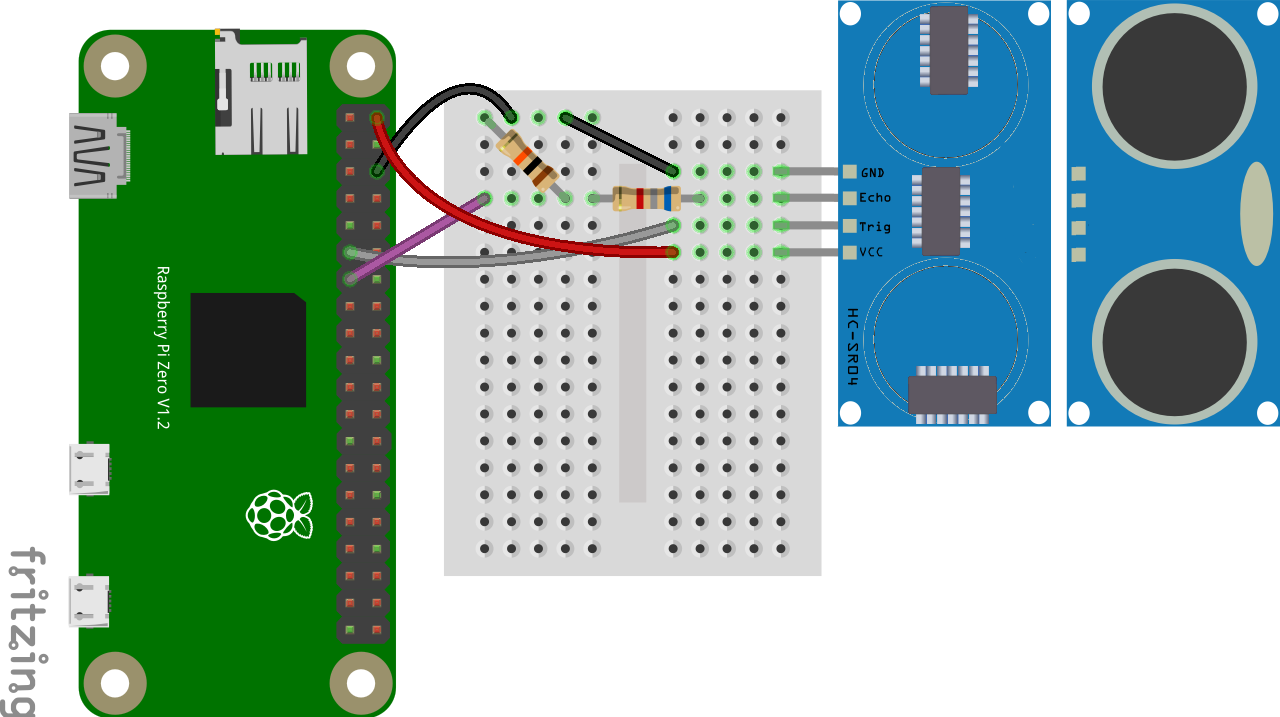
\includegraphics[scale=0.25]{images/HC-SR04_Steckplatine.png}	
  %	\caption{}
  \label{DHT22_Steckplatine}
\end{figure}

%\textbf{Schaltplan:} 

\begin{figure}[ht]
	\centering
	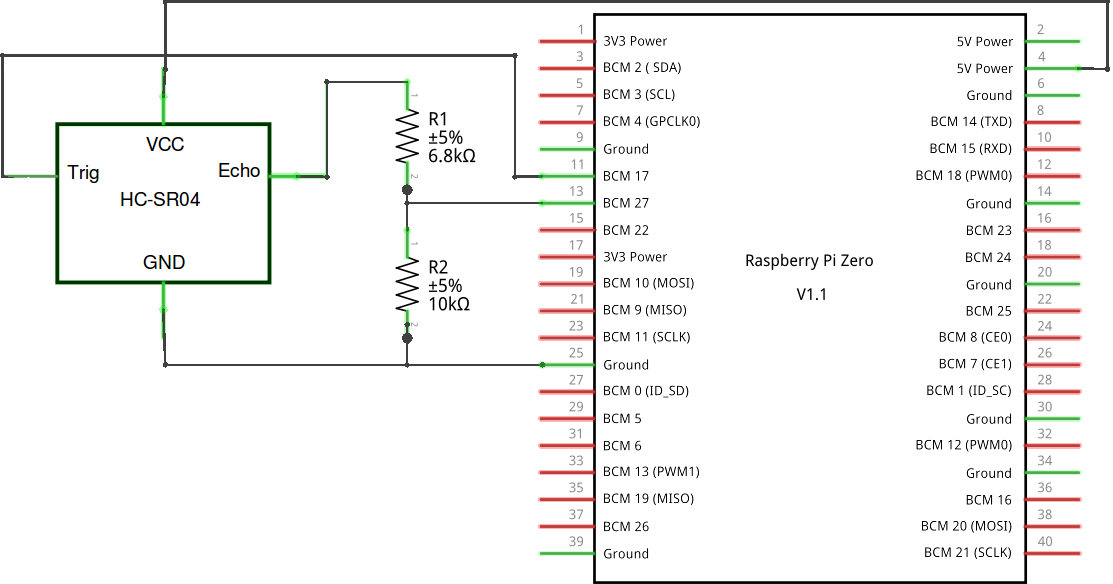
\includegraphics[scale=0.25]{images/HC-SR04_Schaltplan.png}	
	%	\caption{}
	\label{DHT22_Steckplatine}
\end{figure}

\textbf{C:} 

\begin{console}
	git clone https://github.com/mstroh76/HC-SR04Sensor
	cd HC-SR04Sensor
	geany project.geany & 
\end{console}

\textbf{Python:}\\

DistanceSensor.py
\begin{screensmall}
	from gpiozero import DistanceSensor
	from time import sleep
	
	sensor = DistanceSensor(echo=27, trigger=17, max_distance=2.0)
	while True:
		distance = sensor.distance * 100
		print("Distance : %.1f cm" % distance)
		sleep(1)	
\end{screensmall}

\begin{console}
python3 DistanceSensor.py
\end{console}